\section{Ambiente de Programação CHARM++}

\label{charm}
De acordo com os ambientes de programação citados na seção \ref{ambientes-de-programacao-paralela}, o ambiente escolhido para este trabalho é o Charm++. Além das informações descritas sobre ele na seçao \ref{charm-subsection}, a principal razão para sua escolha é  seu framework de balanceamento de carga, que permite tanto criar um novo Balanceador de Carga(BC) quanto utilizar um disponibilizado pelo próprio ambiente de programação.

O Charm++ foi desenvolvido pelo Laboratório de Programação Paralela da Universidade de Illinois, em 1993. Trata-se de uma extensão da linguagem C++, proporcionando um ambiente para programação paralela orientada a objetos. 

De acordo ~\cite{kale1993charm++} Charm++ é basicamente C++ sem suas variaveis globais, com algumas extenções que suportam execução paralela. Operações e manipulações de chares são restritos, em comparação com objetos sequenciais, para se adequear aos requisitos da execução paralela.

\subsection{Chares}
\label{chares}
Para \cite[p.27]{pilla2015programaccao2}, em programas escritos em CHARM++, toda a computação é realizada por objetos especiais chamados de objetos chare. Nesse contexto, objetos chare são similares a threads em OPENMP e processos em MPI, executando de forma concorrente ou paralela em uma plataforma computacional. O conjunto de todos os objetos chare que compõem uma aplicação é chamado de espaço global de objetos. O espaço global de objetos pode mudar durante a execução da aplicação através da criação de novos objetos chare, assim como a deleção dos mesmos.

Os Chares são criados dinamicamente e permitem expressar cálculos onde a criação de tarefas dinâmicas é necessária. Eles podem ser automaticamente mapeados e agendados, proporcionando assim ao usuário capacidades de alto nível. Um chare está agendado para execução apenas quando há uma mensagem disponível para ele. Ao contrário dos processos, os chares não estão executando perpetuamente, nem seu tempo de execução é cortado em processadores. Um chare está sempre pronto para executar qualquer mensagem disponível dirigida a ele~\cite[p.3]{Kale95thecharm}. 

Cada chare conta com seus próprios dados e estado privados, o que implica que outros objetos na aplicação não podem acessar essas informações diretamente. Todo o compartilhamento de dados acontece através da comunicação direta entre chares por troca de mensagens. O modelo de programação permite que um chare se comunique com qualquer outro chare que ele conheça no espaço global de objetos ~\cite[p.27]{pilla2015programaccao2}. A Figura \ref{img-chare} ilustra a interação entre chares citada anteriormente.

\begin{figure}[!htb]
	\centering
	\caption{Comunicação entre os chares A, B e C através de troca de mensagens}
	\centering
    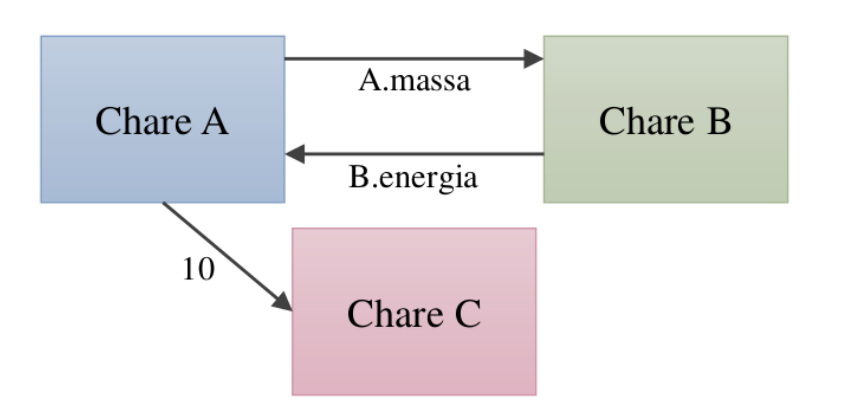
\includegraphics[scale=0.30]{figuras/chares.png}
	\label{img-chare}
    \centering
	\\ Fonte: \cite[p.27]{pilla2015programaccao2}
\end{figure}

Todo programa deve incluir um chare principal que deve ter um ponto de entrada chamado CharmInit. A execução do programa começa pela criação de uma instância do chare principal e a execução de seu ponto de entrada CharmInit ~\cite[p.3]{kale1993parallel2}.

\subsection{Trocas de mensagens}
A troca de mensagens em CHARM++ é feita de forma assíncrona. A troca de mensagens assíncrona faz com que a invocação de um método de entrada em outro chare tenha retorno imediato. Em outras palavras, o chare que envia uma mensagem continu sua execução sem esperar por uma resposta. Adicionalmente, o chare cujo método é chamado pode não começar a executá-lo imediatamente. Esse mecanismo é usado para
guiar a execução da aplicação~\cite[p.28]{pilla2015programaccao2}.

Uma mensagem é uma estrutura constituída por vários campos de dados e é definida de forma semelhante à estrutura de definição em C. As mensagens chegadas são programadas de acordo com uma estratégia de agendamento. A estratégia de agendamento e a estratégia dinâmica de balanceamento de carga são componentes separáveis de modo modular do sistema Charm Runtime, chamado Chare Kernel. O sistema fornece FIFO, LIFO e estratégias de agendamento baseadas em prioridade, com níveis ilimitados de prioridades. Da mesma forma, fornece uma variedade de estratégias dinâmicas de balanceamento de carga desenvolvidas ao longo dos anos. ~\cite{kale1993parallel2}.

Todas as mensagens enviadas para chares em uma unidade de processamento são colocadas em sua fila de mensagens. Cada entrada na fila de mensagens inclui informações sobre qual chare é o receptor, o método invocado e os dados enviados na mensagem ~\cite[p.32]{pilla2015programaccao2}. Como podemos ver na Figura \ref{img-message}. 

\begin{figure}[!htb]
	\centering
	\caption{Distribuição de chares em unidades de processamento e suas filas de mensagens.}
	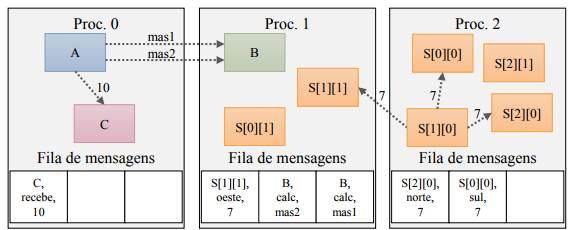
\includegraphics[scale=0.80]{figuras/message.png}
	\label{img-message}
	Fonte: \cite[p.32]{pilla2015programaccao2}
\end{figure}
 
 
 De acordo com ~\cite[p.30]{pilla2015programaccao2} O uso de um modelo de comunicação assíncrona é benéfico pois remove a obrigação de uma sincronização entre o emissor e o receptor de uma mensagem. Isso remove tanto a espera do emissor por uma resposta escondendo parte da latência de comunicação da plataforma quanto o bloqueio da unidade de processamento do receptor enquanto espera pela recepção de uma mensagem.
 
 \subsection{Modelo de execução}
 O processamento nas aplicações em Charm++ é decomposto em objetos chamados chares. O programador implementa as computações e comunicações descrevendo como esses objetos vao interagir e o ambiente de Charm++ gerencia as mensagens geradas por essas interações. Os objetos se comunicam através de chamadas remotas de métodos. Ainda, o ambiente é responsável pelo gerenciamento dos recursos arquiteturais ~\cite{pillaNatalRN}. Na Figura \ref{img-abstracao} podemos ver uma idéa de abstração de aplicação.
 
 \begin{figure}[!htb]
 	\centering
	\caption{Abstração de aplicação na plataforma Charm++}
 	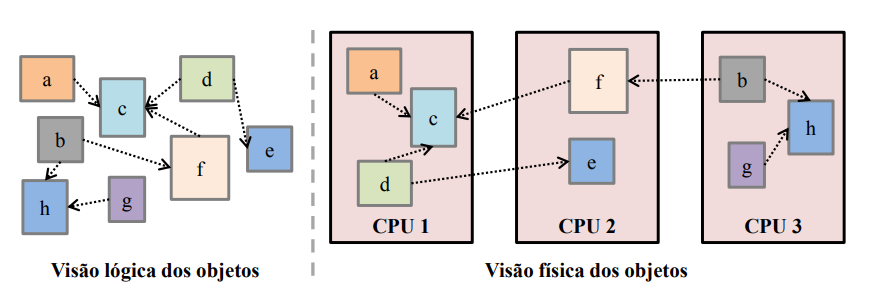
\includegraphics[scale=0.50]{figuras/abstracao.png}
	Fonte: \cite{pillaNatalRN}
 	\label{img-abstracao}
 \end{figure}
 
 No CHARM++, os usuários definem suas aplicações em termos de objetos C++ especiais chamados de chares e coleções indexadas de chares chamados de arrays de chare. Para a maioria, os conjuntos de chares e chare são definidos exatamente como classes padrão e arrays C++, permitindo que o programador aproveite o encapsulamento e abstração de dados. Normalmente, há muitos mais chares do que PEs(processing elements), permitindo que o RTS(Runtime System) aproveite a composição. Como o CHARM ++ usa um paradigma baseado em objetos, o programador também pode implementar facilmente diferentes tipos de unidades de trabalho ~\cite{acun2014parallel}.
 
 No momento em que um projeto do Charm++ é compilado além dos arquivos de cabeçalho com extensão .h e os códigos padrões com extensões .C por exemplo,  o compilador do Charm++ denominado CHARMC utiliza um tradutor que faz a leitura do arquivo de interface. Após a leitura do arquivo de interface são gerados 2 arquivos com extensões .def.h e .decl.h. Após essa etapa o compilador é utilizado novamente para gerar o arquivo de saída com extensão .o. Para rodar a aplicação é necessário utilizar um arquivo de execução do próprio Charm denominado CHARMRUN. Este Fluxo pode ser visto na Figura \ref{img-compiler} a seguir:
 
 \begin{figure}[!htb]
	\centering
	\caption{Processo de compilação de um projeto utilizando CHARM++}
	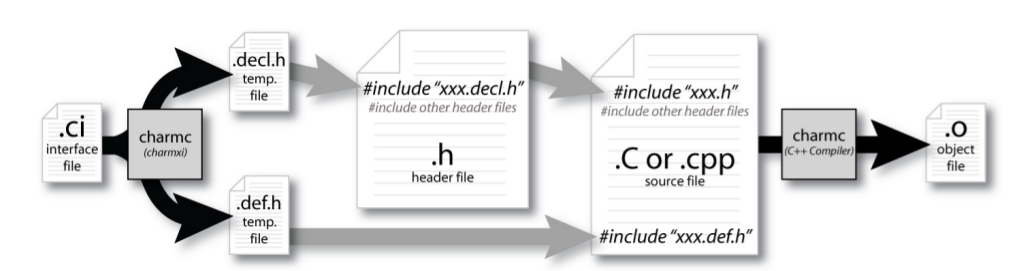
\includegraphics[scale=0.40]{figuras/compile.png}
	\\ Fonte: \cite{compileIMG}
	\label{img-compiler}
\end{figure}

\subsection{Balanceamento de carga}

Muitas estratégias de balanceamento de carga em CHARM++ são baseadas em uma heurística conhecida como princípio da persistência. Ele postula que, empiricamente, para certas classes de aplicações científicas e de engenharia, quando elas são expressadas em um termo de objetos naturais, as cargas computacionais e padrões de comunicação tende a persistir ao longo do tempo, mesmo em cálculos com evolução dinâmica~\cite{zheng2010hierarchical}.
%Many load balancing strategies in CHARM++ are based on a heuristic known as the principle of persistence. It posits that, empirically, for certain classes of scientific and engineering applications, when they are expressed in terms of natural objects (as CHARM++ objects or threads), the computational loads and communication patterns tend to persist over time, eve in dynamically evolving computations. This has led to the development of measurement-based load balancing strategies that use the recent past as a guideline for the near future

De acordo com \cite{pilla2015programaccao2}, O balanceamento de carga em CHARM++ é baseado na medição do tempo de atividade dos chares e das unidades de processamento. Durante um certo período de execução de uma aplicação, o sistema coleta uma serie de informações , esses dados são organizados pelo ambiente em um vetor de informações sobre chares e um vetor de informações sobre unidades de processamento, os quais são encaminhados a um algoritmo de balanceamento de carga. O algoritmo é responsável por avaliar as informações atuais recebidas e prover um novo mapeamento de chares para unidades de processamento. Para habilitar o balanceamento de carga em uma aplicação em CHARM++, o programador é responsável apenas por implementar métodos de serialização para os objetos, por inserir uma chamada ao método bloqueante AtSync() em algum momento da execução de todos os chares e por definir um método de entrada ResumeFromSync(), o qual será chamado após o término do balanceamento de carga. Quando todos os chares alçarem a chamada AtSync, um algoritmo de balanceamento de carga externo, o qual foi compilado em anexo à aplicação e escolhido no momento de sua execução, computará um novo mapeamento.

%Depending on the needs of applications, the user can invoke appropriate load balancer. The load balancing framework in CHARM++ instruments each chare as well as records the PE’s load. In the AtSync mode of load balancing, all the chares pause their execution and call AtSync. The load statistics are collected and the user specified load balancing strategy is used to compute the new mapping. Once the load balancing decision is made, the framework handles the migration of the chares to the newly mapped PEs and resumes them.

 